\chapter{Results and Discussion}
\section{Final Design}

\begin{figure}[h]
    \centering
    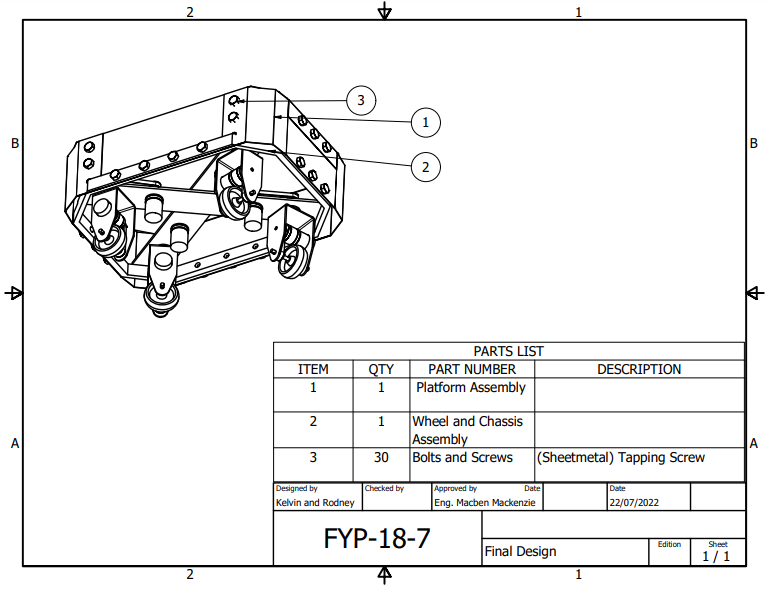
\includegraphics[scale = 0.7]{Figures/NewFinalAssemblyParts.png}
    \caption{Final Design}
    \label{fig:finalassemblyparts}
\end{figure}

\begin{figure}[h]
    \centering
    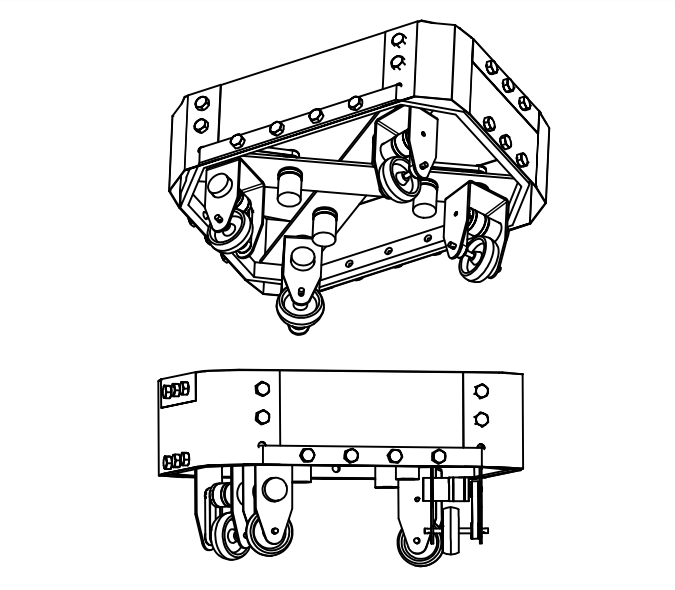
\includegraphics[scale = 0.8]{Figures/NewFinalDesignDWG.png}
    \caption{Final Assembly}
    \label{fig:finalassembly}
\end{figure}

\section{Load analysis on Platform}

\begin{figure}[H]
    \centering
    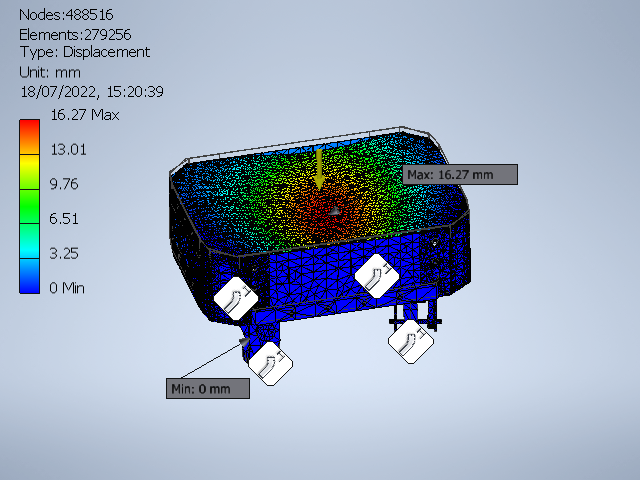
\includegraphics[scale = 0.9]{Figures/PlatformDisplacement.png}
    \caption{Displacement by Load}
    \label{fig:platformdisplacement}
\end{figure}

A force of $400N$ was applied on the platform top to simulate a practical load of $40kg$ on the platform. The results indicate a displacement of $16.27mm$ in the Z-axis at the point of application. However, since the load will be distributed evenly on the platform surface this displacement will be evenly distributed along the platform and won't be as apparent practically.
\par
This displacement will also be alleviated by adding a support shaft that rests on the chassis. The analysis also suggested a maximum safety factor of $15$ as shown on Figure \ref{fig:safetyfactor} on areas that receive little force and a safety factor of between $3$ and $6$ for the top of the platform. This allows a force up to six times the base force of $400N$ before the platform fails.

\begin{figure}[H]
    \centering
    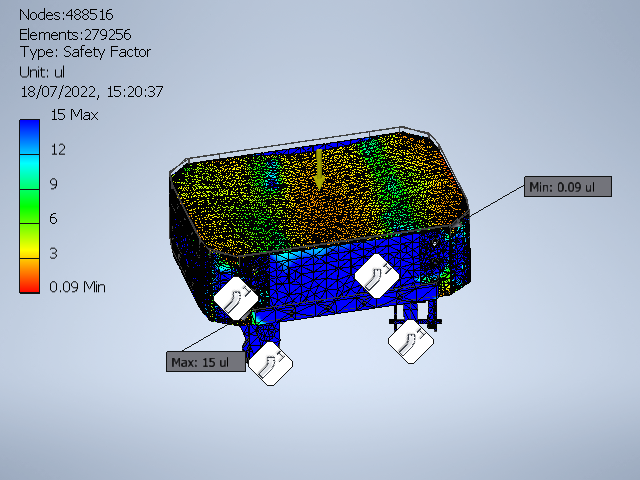
\includegraphics[scale = 0.9]{Figures/safety_factor.png}
    \caption{Safety Factor}
    \label{fig:safetyfactor}
\end{figure}

\section{Load analysis on Chassis}

\begin{figure}[H]
    \centering
    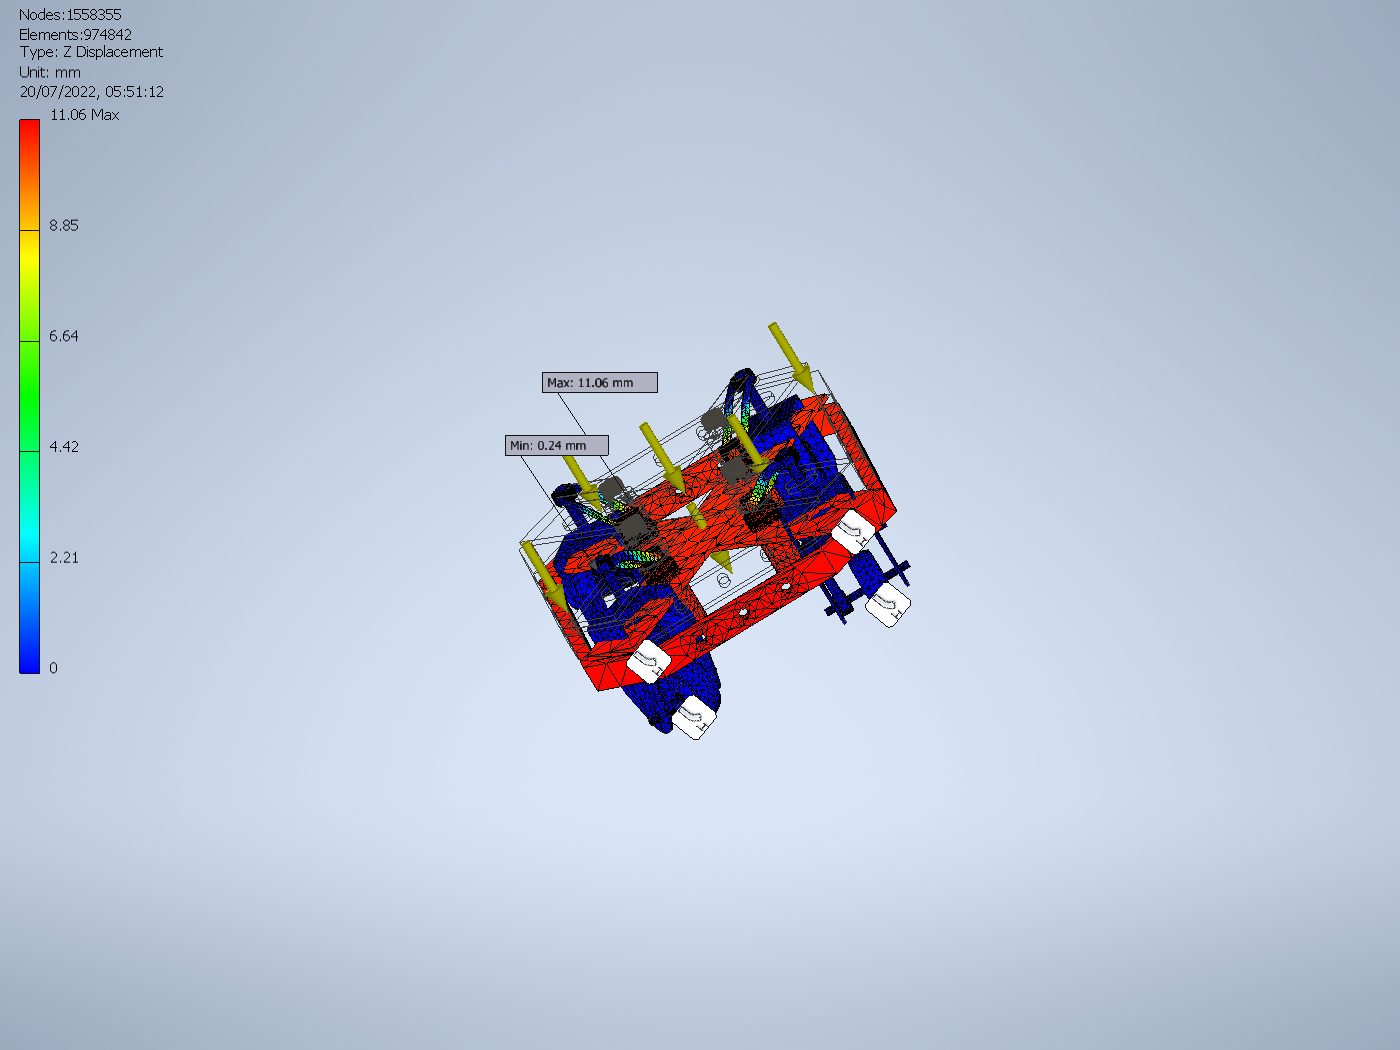
\includegraphics[scale = 0.4]{Figures/ChassisDisplacement.png}
    \caption{Displacement of Chassis by load}
    \label{fig:chassisdisplacement}
\end{figure}
\par
The analysis results showed that the chassis can handle the maximum load desired, albeit a displacement of $11.06mm$. This displacement is concentrated at the centre of application of the force, but since the force will be evenly distributed across all chassis faces, the expectation is that the displacement will be minimum. The chassis should comfortably carry the weight.

% \section{Torque analysis on Wheel Frame}

% \begin{figure}[H]
%     \centering
%     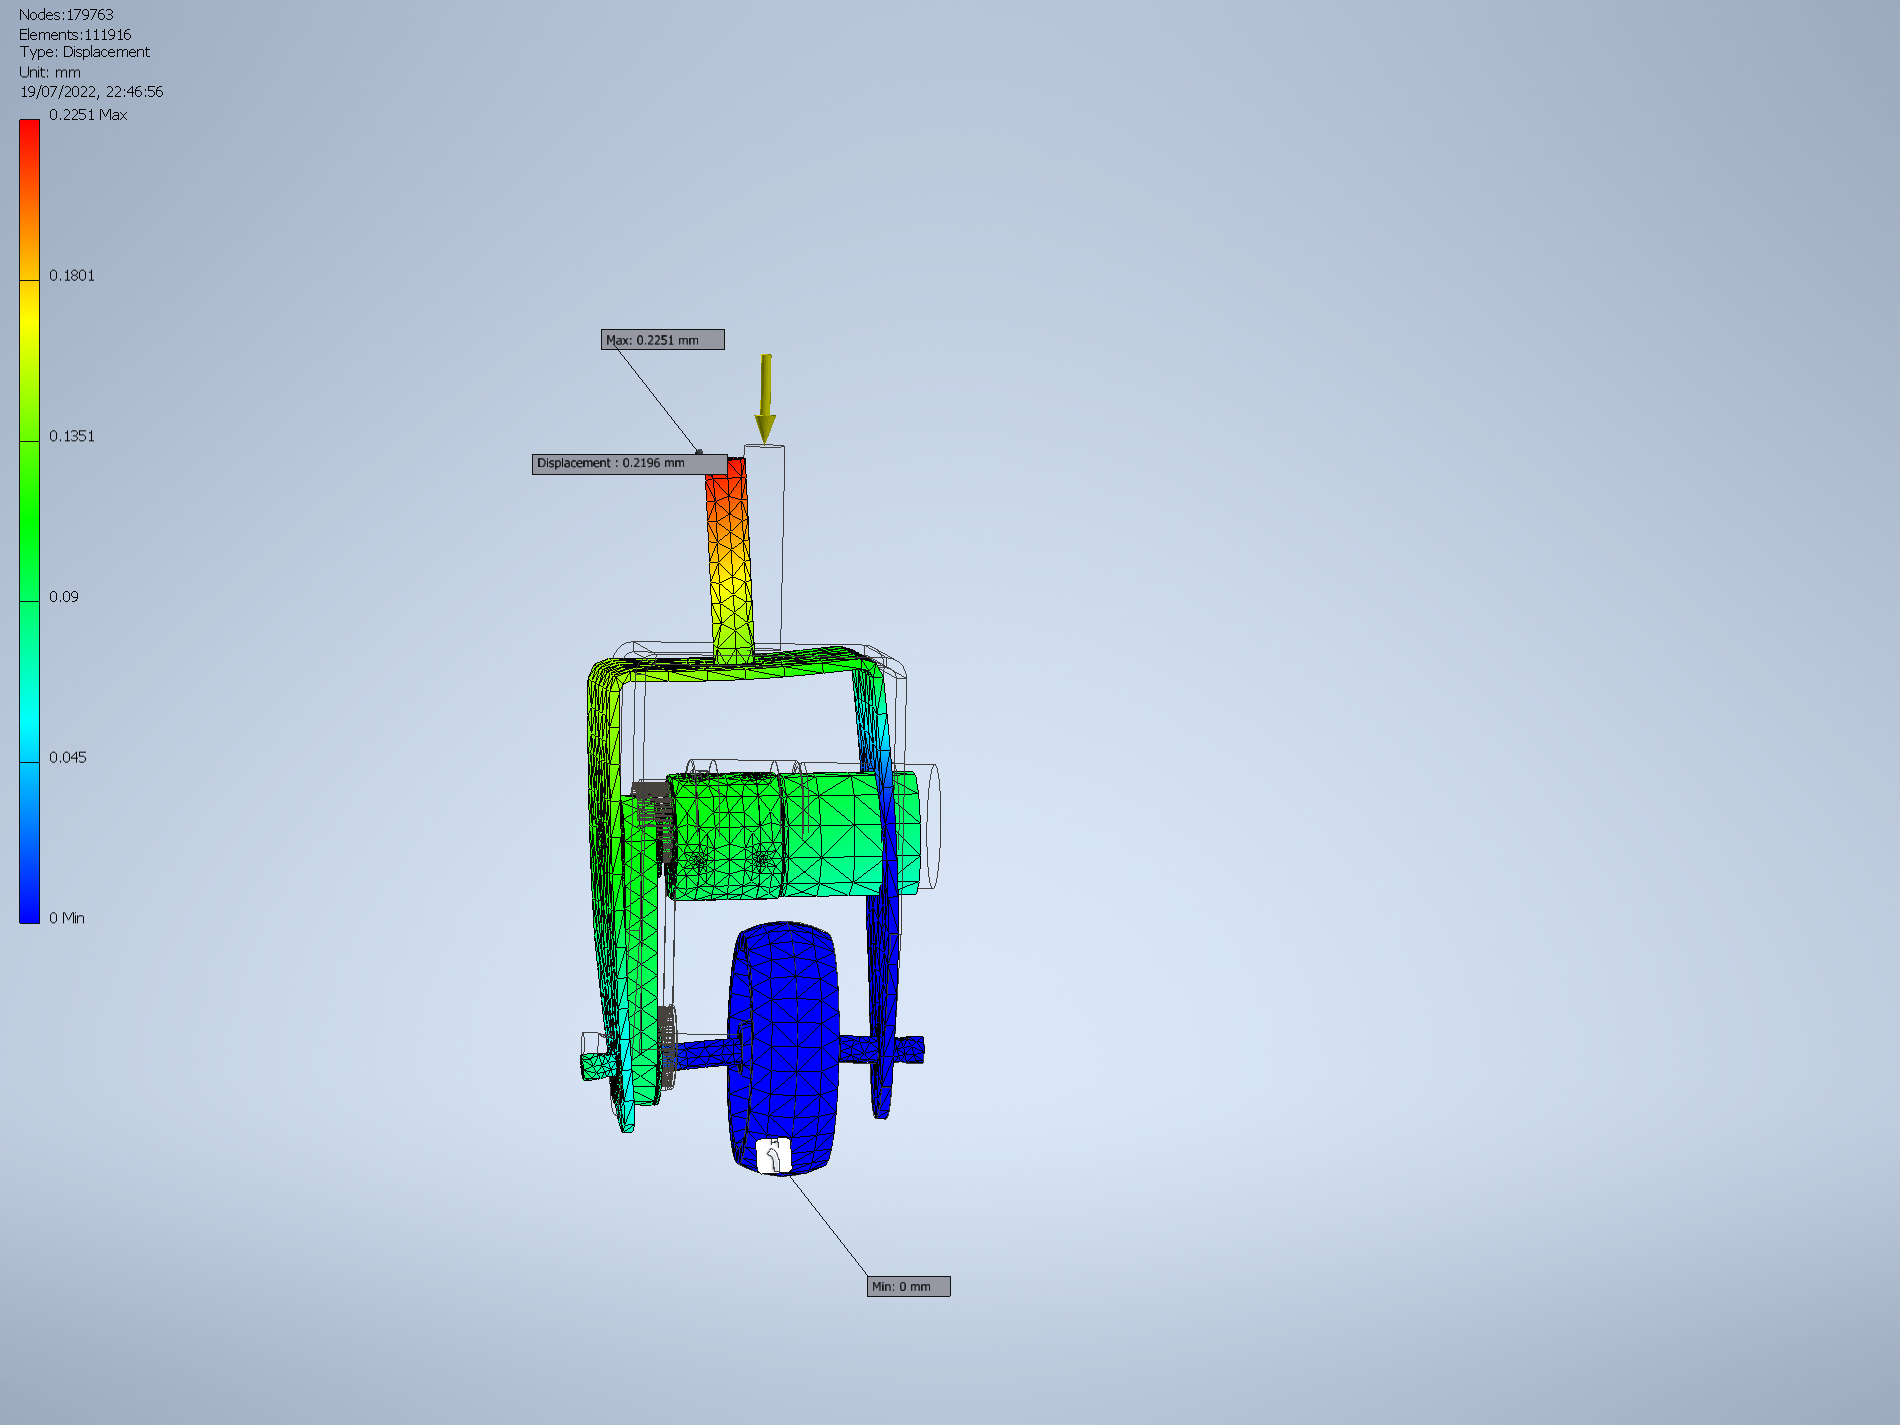
\includegraphics[scale = 0.3]{Figures/WheelFrameDisplacement.png}
%     \caption{Load Displacement on Wheel Frame}
%     \label{fig:wheelframedisplacement}
% \end{figure}

% \section{Motor control analysis}
% TO BE ADDED

\section{Budget}
\begin{table}[H]
  \begin{center}
    \leavevmode
    \hangcaption[Cost Budget]{Cost Budget}
     \begin{tabular}{| l | c | c | c | c | c |}\hline
No. & Item & Quantity & Supplier & Unit Cost & Total cost \\\hline
1 & Satima S2 Motor driver & 4 & Pixel Electric & 500 & 2000 \\\hline
2 & STM32F103C8T6 & 1 & Nerokas & 1000 & 1000 \\\hline
3 & MPU-6050 & 1 & Nerokas & 260 & 260 \\\hline
4 & Esp 12 F & 2 & Nerokas & 300 & 600 \\\hline
5 & Passive components & 1 & Pixel Electric & 1000 & 1000 \\\hline
6 & PCB & 2 & & 500 & 1000 \\\hline
7 & 18650 Lithium Ion Battery & 5 & Pixel Electric & 350 & 1750 \\\hline
8 & DC motor & 8 & Pixel Electric & 1100 & 8800 \\\hline
9 & Motor Bracket & 8 & Pixel Electric & 300 & 2400 \\\hline
10 & Motor shaft and couplings & 4 & Pixel Electric & 200 & 800 \\\hline
11 & Bearing & 4 & Hardware & 100 & 400 \\\hline
12 & V-belt pulley & 16 & Pixel Electric & 150 & 2400 \\\hline
13 & Belt & 8 & Hardware & 200 & 1600 \\\hline
14 & Castor Wheels & 4 & Nerokas & 200 & 800 \\\hline
15 & Steel rods & 5 & Hardware & 60 & 300 \\\hline
16 & Aluminium Sheet & 1 & Hardware & 600 & 600 \\\hline
17 & Fasteners & 1 & Hardware & 500 & 500 \\\hline
18 & Miscalleneous & 1 & & 2600 & 2600 \\\hline
& & & & & \\\hline
& & & & TOTAL & 28810 \\\hline
    \end{tabular}
    \label{table:1}
  \end{center}
\end{table}


\begin{table}[H]
  \begin{center}
    \leavevmode
    \hangcaption[Power Budget]{Power Budget}
     \begin{tabular}{| l | c | c | c | c |}\hline
Component & Voltage (V) & Current (mA) & No. of Components & Power (W) \\\hline
MPU6050 & 3.3 & 4.68 & 1 & 0.015444 \\\hline
ESp32 & 3.3 & 480 & 1 & 1.584 \\\hline
Stm32 & 3.3 & 360 & 1 & 1.188 \\\hline
Led & 3.3 & 120 & 2 & 0.792 \\\hline
DC motor & 12 & 360 & 8 & 34.56 \\\hline
Motor driver & 5 & 43.2 & 1 & 0.216 \\\hline
& & & & 38.355444 \\\hline
    \end{tabular}
    \label{table:1}
  \end{center}
\end{table}


% With a $3.2 Ah$ battery we will be able to run the mobile platform for 1hr without charging. Since we don’t have that, the available battery would be a $2.8 Ah$ battery that would’t raise the cost that much further.

% \begin{equation} \label{totalefficiency}
% \begin{split}
% t & = \frac{2.8}{3.2288}\\
% & = 40 mins 53s
% \end{split}
% \end{equation}

% With a $2.2 Ah$ battery we are now able to run for approximately $40 mins$
